\paragraph{Overview} The aim of the Airdrop system is to deliver a Unmanned Ground Vehicle (UGV, same as Rover) to a designated location and also provide real time images to the ground using on-board computer and communication modules. For the delivery, after the waypoint capture mission, which may goes up to 4 miles in distance, Condor will arrive at the drop location that is previously given to us. Then the payload system will lower the Rover while the aircraft stays loitering, and use a pulley system to release the Rover autonomously before retrieving the rope. Then the system will idle until the end of the mission. For the image transfer task, after the aircraft enters the search area, the camera will start taking images at a preset interval while the aircraft is at this specific flight area. The image is tagged on-board with the real-time data from flight controller and then transferred to the GCOMv2 server computer immediately.  
% read
\paragraph{System Component}
Payload system consist of 3 parts: 
\begin{itemize}
    \item Imaging system, UGV and air delivery system.  The imaging system has a camera, 1 axis gimbal, raspberry pi, bullet, POE ejector and image transferring software. 
    \item Rover consists of UGV, UGV control software and water bottle. 
    \item Air delivery system has a Winch, winch control electrical system, winch control software and various hardware to mount UGV. 
\end{itemize}
%read


\subsubsection{Winch subsystem}
\paragraph{Requirements}
The requirements of the winch subsystem were based on the aircraft's capability and competition's operation and flight time window. 
\begin{itemize}
    \item Weight cannot exceed 1 kg.
    \item Power consumption: limited to 5V and 12V, parallel to the aircraft's PCB.
    \item Operate at the minimum competition flight attitude, which is 30m MSL.
    \item Can withstand 5G acceleration, up to 25m/s.
    \item Complete the whole airdropping operation under 1 minute.
\end{itemize} 

The team considered three designs for deploying the UGV from Condor: parachute drop, pulley system or a direct drop. A direct drop was eliminated from the list as Condor has a minimum altitude - one that is too high to safely drop the. Since the parachute is the lightest option when considering weight, the team tested it by prototyping different types and designing one that yields the highest precision on its drop location. It needs to be ensured the rover is dropped at sufficiently low velocity. The velocity attained via the parachute was too high to merit a safe drop. Additionally, a parachute would require the UGV to be encompassed with some protective material to survive the drop, which would ultimately cause the 1kg UGV weight limit to be exceeded. Testing revealed the parachute to be too unpredictable and difficult to control. Thus, a pulley system was designed. The pulley can control the releasing speed of the 1kg UGV from the lowest flight altitude.
%read

\paragraph{Design Consideration}
The winch system has two tasks: release the Rover and retract a rope. The first task uses a servo controlled brake and motor drag system, and the second task uses the same motor to recover the rope. Both systems are dependent on an encoder to measure the length of the rope used. %read

The winch system is designed based around limiting the rotating drum’s maximum RPM (Revolutions Per Minute) to obtain precise measurement of length and instant velocity and to minimize the weight. To find the size of the drum, it was first assumed that releasing and retracting will take 15 seconds and 5 second each from a 30 meter drop height. During prototyping, our first iterations encoder worked the best at around 400 RPM, however later on a better encoder that raised the RPM cap to over 1000 was acquired. When determine the retracting RPM, it was found that when over 600 RPM, the rope will start over-retracting and cause rope interleaving; slower RPM leads to longer retracting time and motor under-powering. Drum size was based on estimating the diameter x with: $$600 RPM \cdot \frac{15s}{60s} \cdot (x cm \cdot \pi) = 3000 cm$$ which results in about 6.3 cm in diameter. 
%read

Next a gear train was designed to make sure that the RPM for the encoder was within its optimal measurement range. For this stage Cylewet’s CLT1062 encoder was used, which provides 20 pulses or 40 ticks per revolution. This relatively cheap and light encoder was elected based on estimations of system limitations. Considering the worst case of free falling for 20 meters, which result in about 20m/s of velocity:
$$20 m/s \rightarrow 2,000 cm/s \rightarrow 2 cm / ms \approx  0.1 resol/ms \rightarrow 4 ticks/ms$$
Given the maximum reading frequency of the Teensy Encoder module of 50kHz, which is less than 1 ticks/ms, it was decided that the encoder did not need to be geared down.

As for choosing the motor, a DC motor was chosen over a stepper motor due it’s light weight and faster no load RPM. Although a stepper motor gives full control over the releasing with it’s high stall torque($\approx$ 1.5kg * 6.3 cm ~ 9.45 kg cm), with the voltage and current limitation, the stepper motors that meets this requirement are at least 500 grams. In addition it's low RPMs are not able to meet the operation time window. Therefore the following motors were tested: (RPM/stall torque) 300 RPM/15kg$\cdot$cm, 1k RPM/6kg$\cdot$cm, 3.5k/3kg$\cdot$cm and 10k RPM/3kg$\cdot$cm. It was found that the 1k RPM with 6 kg$\cdot$cm stall torque motor can meet the retracting speed requirement and at the same time provides noticeable slow down when releasing. The drum motor was geared up by 1.4 to give more control over the retracting. To compensate for motor’s low stall torque, a servo trigger friction brake was added that is capable of stopping the drum with only 30 cm delay after a 2 second free fall.
Refer to Table 3 for specific measurements. 

\begin{figure}[h]\centering
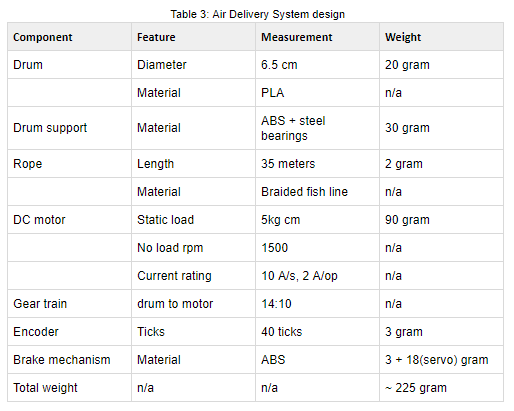
\includegraphics[width=\linewidth]{table/Table_3_Air_delivery_system_design.PNG}
\caption*{}
\label{fig:airdrop_design}
\end{figure}



\paragraph{Operation}
The winch subsystem has two modes: manual mode allows the pilot to trigger the winch mechanism using a channel switch on the flight controller where as autonomous mode gets triggered automatically when the quadcopter reaches the desired GPS location. On the flight side, the on-board computer (Raspberry Pi 3) triggers the winch operation. The Teensy 3.5 microcontroller begins the releasing operation - it sets a servo based braking mechanism to its release position, and the motor is powered at the same time to generate a counter torque. A rope is released, whose length is measured with a rotational encoder. The encoder measures the rotational resolutions of the drum and calculates the approximated distance and instant velocity of the releasing. If the dropping speed exceeds a certain threshold, the braking system and motor will adjust the error with a PD controller. Once the winch system has detected that the Rover has reached the ground or the releasing altitude has met the length of the rope released, a linear actuator will release the geared slider on the Rover and detach the rope. The rope is then retracted back to the aircraft, finishing up the airdrop operation in a physically and electrically stable state. 
%read

\begin{figure}[h]\centering
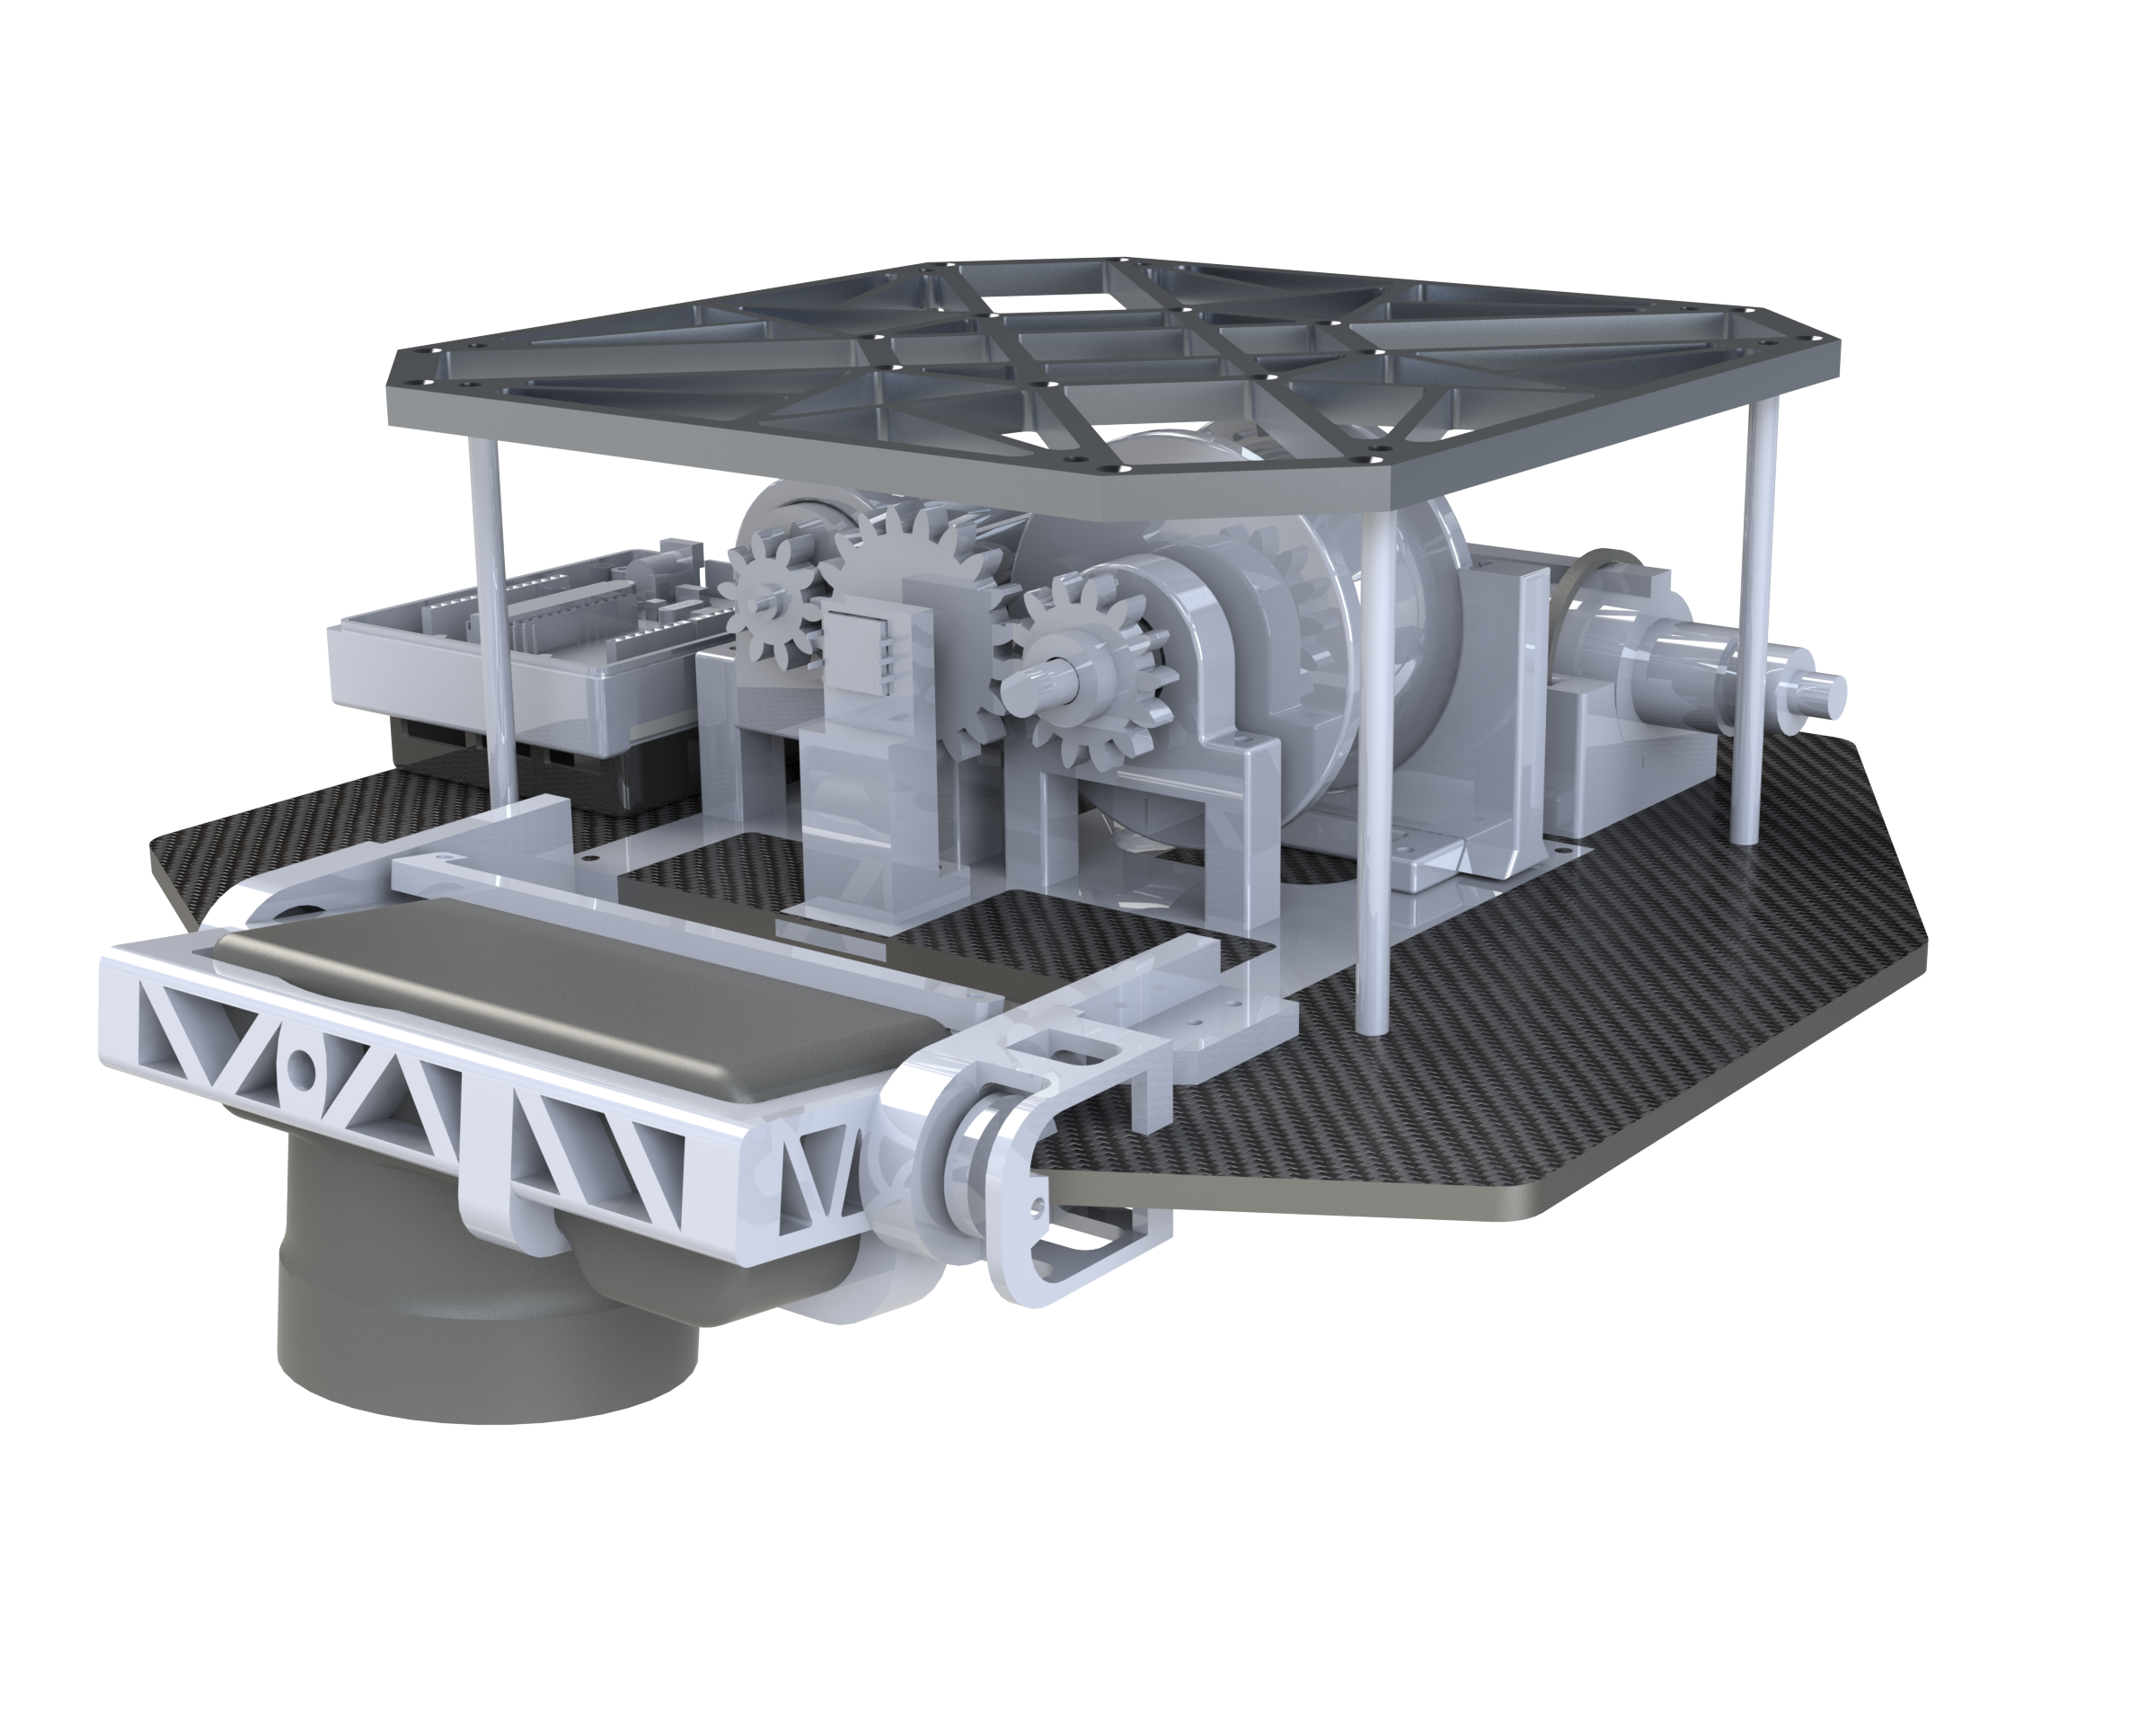
\includegraphics[width=\linewidth]{figures/PayLoad.png}
\caption{Winch subsystem Diagram}
\label{fig:winch_diagram}
\end{figure}

\paragraph{Testing}
To test the winch system, first an isolated testing environment was set up to make sure that each components work as expected, then they were integrated with a testing aircraft and finally Condor. After each component was tested, an integrated test to select the releasing algorithm and controllers was conducted by releasing a similar payload from a high altitude location (A 3rd floor sundeck), and the performance of the dropping was recorded. In the end, it was found that the system can be controlled only with a proportional differential(PD) controller.  

For aircraft testing, the testing multirotor was set to loiter at 30 meters and the winch underwent several tests with various dropping speed, different controller algorithms and dropping altitudes ranging from 20 to 40 meters. The ground personnel observed and recorded the dropping accuracy, the stability of the drop and the integrity of the payload. In the end it was concluded that 15 seconds dropping window not only feasible, but also was the configuration with one of the most stable performances, as the aircraft wasn't as influenced from the rapid controller error correction and the drop was efficient due to it's relatively short drop time. Although the oscillation created at the end of the 30 meter long rope only seems to be a major problem in windy weather, some manual tuning on the PD controller will be conducted on site depending on the wind conditions, since the winch can reliable perform a high speed drop and completely stop the release within about half a meter from a 2 second free drop. 
%read

\subsubsection{Unmanned Ground Vehicle}
\paragraph{Requirements} 
We set design requirements for the rover to meet or exceed the competition requirements. 
\begin{itemize}
\item The weight is not to exceed 1 kg, with the water bottle attached. 
\item The rover should autonomously drive to a specified location.
\item In case of loss of communication or driving out of specified boundaries, the rover is to stop driving within 30 seconds. 
\item The speed of the rover is limited to 10 miles per hour.
\end{itemize}

To meet these requirements of autonomy and emergency shutoff, it was additionally required that the rover contain a GPS receiver, radio receiver, and motor controller. 

\paragraph{Design Process and Mechanism Description} 
Besides the performance goal of delivering a water bottle, a great deal of freedom was awarded in designing the rover. Prototypes with three wheels and four wheels, and a variety of attachment systems to secure the rover to the UAV in flight were considered. Ultimately, the decision to use four wheels was made. This allowed the team to design a smaller base-plate and a shorter rover, since the water bottle can be positioned between the wheels (See Figure 6). Furthermore, having four wheels improves stability, which is greatly beneficial on uneven terrain. A rack-and-pinion design at the top of the rover was used for the detachment mechanism, which was chosen for its reliability in actuation. The rack was modified to allow for the rover to attach at three non-collinear points, which increases resistance to vibrations and changes in direction during flight. 

3D printing was harnessed extensively to perform rapid prototyping and to achieve tight fits around other electronic components, which would not have been feasible with traditional manufacturing methods. As a result, as shown in the diagram below, the rover’s components are packed tightly into a space-efficient design (Figure 7).

\begin{figure}[H]\centering
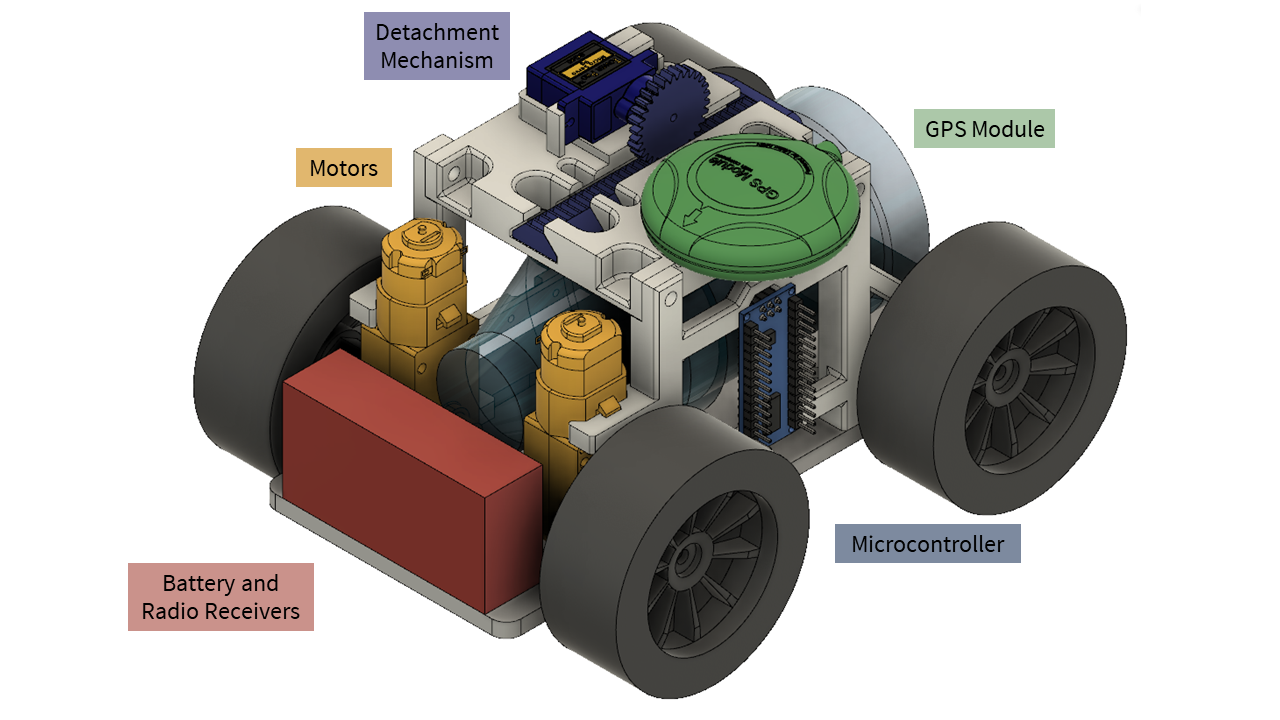
\includegraphics[width=\linewidth]{figures/Rover_Diagram.png}
\caption{Rover subsystem Diagram}
\label{fig:systems_link_diagram}
\end{figure}

\paragraph{Testing Methods} 
The performance of the rover system itself was tested by letting it drive autonomously to specified GPS coordinates in a field. To test the rover as a component of the entire payload system, the detachment mechanism was first tested by flying the UAV at a low height and lowering the rover, and eventually flying the UAV in normal operating speeds and accelerations and testing that the rover could withstand the vibrations and changes in direction typical to UAV flight.

\endinput

